% Drawing 142/04-1 -- folder 142, batch 04, archive page 61 (PDF page 62).
% Transcription: En haut à gauche, une sphère : pôle nord $P_+$, pôle sud $P_-$ ; sur l'équateur, de gauche à droite, $Q_1$, $R_0^-$, $R_0^+$, $Q_\infty$, $R_1^-$ ; deux petits cercles sur l'équateur, l'un entre $R_0^-$ et $R_0^+$ (avec $S_0^+$ au-dessus, $S_0^-$ au-dessous), l'autre près de $R_1^-$ (avec $S_1^+$) ; des méridiens joignent $P_+$ à $P_-$ ; un fuseau hachuré sous $P_+$, marqué d'une flèche circulaire d'orientation.
% Kind: sphere with poles, meridians, small circles and a hatched lune. Method 2 (schematic redraw from the facsimile). Status: partial.
% Notes: Pencil outline; P_+ at the top, P_- at the bottom; meridians from P_+ (inked) to the equator and on to P_-; on the equator, left to right, Q_1, R_0^-, R_0^+, Q_infty, R_1^-; a small circle between R_0^- and R_0^+ (S_0^- below), another near R_1^- (S_1^+ above), and a small ring above R_0^+. The hatched lune under P_+ with its circular orientation arrow. The lower half is faint and only partly drawn.
% Coordinates: 1 unit = 1 mm = 1/100 of the crop width (bbox in page fractions: [0.12, 0.07, 0.29, 0.22]).
% Redrawn by Claude (claude-opus-5-5), issue #73, 2026-11-07; not checked by a human; not compiled (no TeX in the session).
% Rights: reproduces part of the work -- behind RENDER_TRANSCRIPTS, never published by itself.
\documentclass[tikz,border=3pt]{standalone}
\usepackage{amsmath,amssymb}
\usetikzlibrary{patterns,arrows.meta}
\tikzset{pencil/.style={black!45}, struck/.style={black!35}, mark/.style={circle,draw,inner sep=1.3pt}, pt/.style={circle,fill,inner sep=0.9pt}, opt/.style={circle,draw,fill=white,inner sep=1.1pt}}
\begin{document}
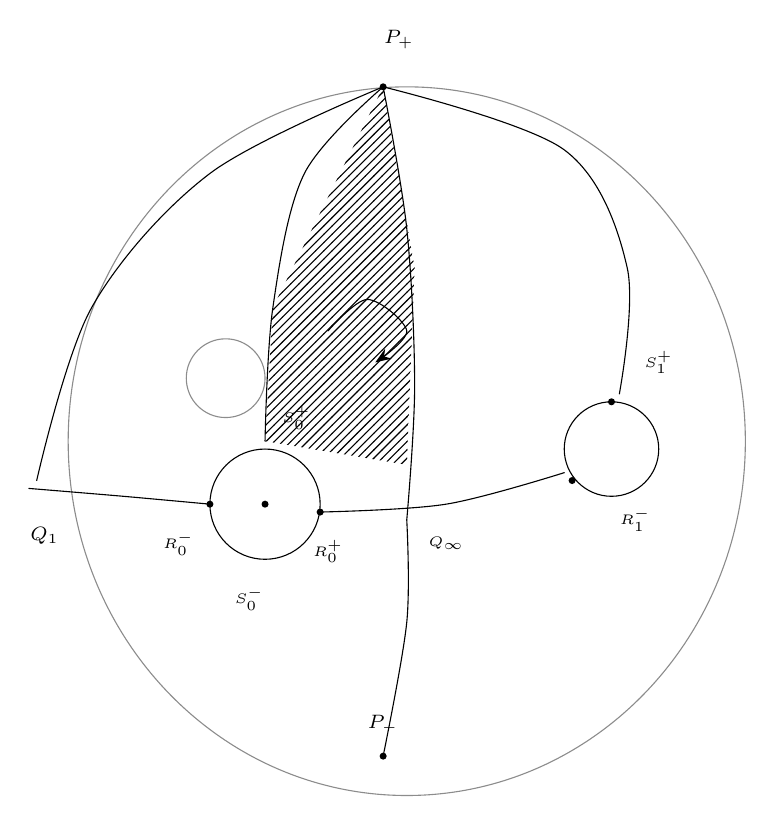
\begin{tikzpicture}[x=1mm,y=1mm,line cap=round,line join=round,font=\scriptsize]
\draw[pencil] (50,-72) ellipse[x radius=43, y radius=45];
\node[pt] at (47,-27) {};
\node[pt] at (47,-112) {};
\draw plot[smooth, tension=0.55] coordinates {(47,-27) (25,-38) (10,-55) (3,-77)};
\draw plot[smooth, tension=0.55] coordinates {(47,-27) (37,-38) (33,-55) (32,-72)};
\draw plot[smooth, tension=0.55] coordinates {(47,-27) (50,-45) (51,-65) (50,-82)};
\draw plot[smooth, tension=0.55] coordinates {(47,-27) (70,-35) (78,-50) (77,-66)};
\draw plot[smooth, tension=0.55] coordinates {(50,-82) (50,-95) (47,-112)};
\fill[pattern=north east lines] (47,-27) -- (33,-55) -- (32,-72) -- (50,-75) -- (51,-50) -- cycle;
\draw plot[smooth, tension=0.55] coordinates {(2,-78) (14,-79) (25,-80)};
\draw plot[smooth, tension=0.55] coordinates {(39,-81) (55,-80) (70,-76)};
\draw (32,-80) circle[radius=7];
\draw[pencil] (27,-64) circle[radius=5];
\draw (76,-73) circle[radius=6];
\node[pt] at (32,-80) {};
\node[pt] at (25,-80) {};
\node[pt] at (39,-81) {};
\node[pt] at (76,-67) {};
\node[pt] at (71,-77) {};
\draw[-{Stealth[length=2mm]}] plot[smooth, tension=0.55] coordinates {(40,-58) (45,-54) (50,-58) (46,-62)};
\node[inner sep=1pt] at (49,-21) {\scriptsize $P_{+}$};
\node[inner sep=1pt] at (47,-108) {\scriptsize $P_{-}$};
\node[inner sep=1pt] at (4,-84) {\scriptsize $Q_1$};
\node[inner sep=1pt] at (21,-85) {\tiny $R_0^{-}$};
\node[inner sep=1pt] at (40,-86) {\tiny $R_0^{+}$};
\node[inner sep=1pt] at (55,-85) {\tiny $Q_\infty$};
\node[inner sep=1pt] at (79,-82) {\tiny $R_1^{-}$};
\node[inner sep=1pt] at (30,-92) {\tiny $S_0^{-}$};
\node[inner sep=1pt] at (36,-69) {\tiny $S_0^{+}$};
\node[inner sep=1pt] at (82,-62) {\tiny $S_1^{+}$};
\end{tikzpicture}
\end{document}
